\documentclass[a4paper,11pt]{article}
\usepackage[left=1.5cm, right=1.5cm, top=2cm, bottom=1.5cm]{geometry}
\usepackage{graphicx}
\usepackage{amssymb}
\usepackage{amsmath}
\usepackage{wrapfig}

\begin{document}
\title{\LARGE{\textbf{ECEN 204 Design Report}\\Power Supply}}
\author{Niels Clayton : 300437590\\ \textbf{Lab Partner: }Nickolai Wolfe}
\date{September 15, 2019}
\maketitle
\hrule

\section{Introduction}
Most electrical devices require an external power supply in order to function.  In a New Zealand household, this power will be sourced from the 50Hz, 240V AC (alternating current) wall outlet. However most electrical devices require a much lower DC (direct current) voltage to operate correctly. To convert between this high voltage AC input and low voltage DC output a power supply can be used. This report will look at the aspects of a simple 12V AC to 5V DC power supply, and discuss possible design choices.

\subsection{Power Supply fundamentals}

\begin{figure}[h]
 \begin{center}
  \fbox{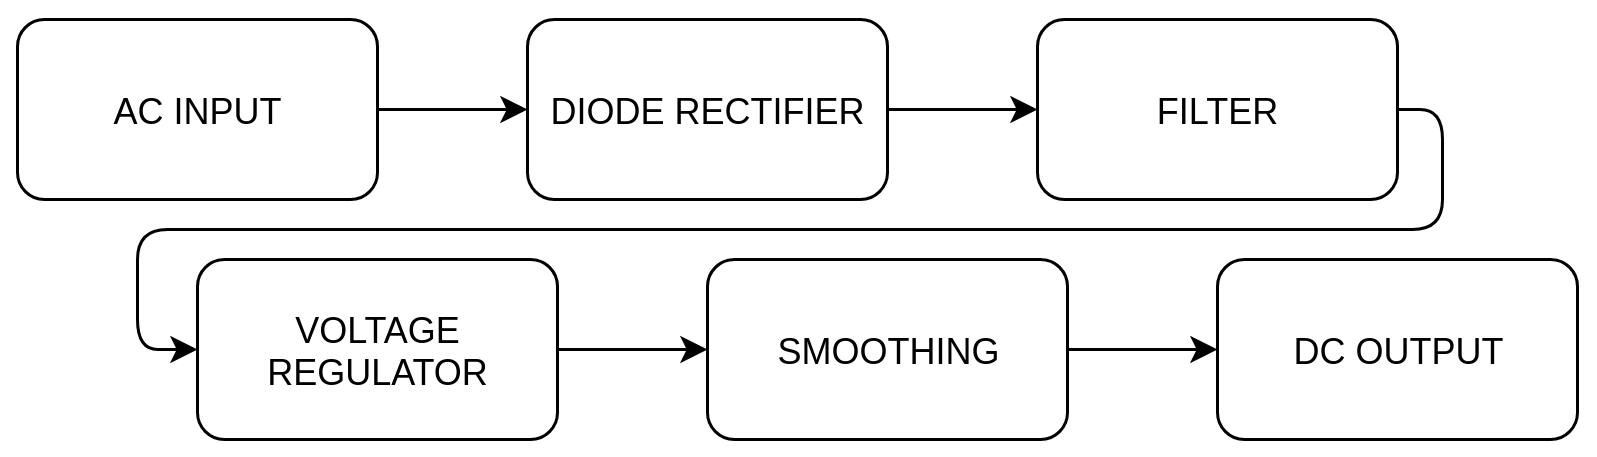
\includegraphics[width = \textwidth]{Images/Diagram.png}}
  \caption{Fundamental building blocks of a power supply}
 \end{center}
\end{figure}

Figure 1 shows the basic design of an AC to DC power supply, broken into the fundamental building blocks. The following section will expand upon the purpose of each of these. 

\subsubsection{AC Input}
The input voltage source for this projects power supply will be standard 240V, 50Hz AC. AC voltage oscillates as a sinusoidal signal, leading to both positive and negative currents. The AC input voltage will also need to be 'stepped down' to a lower voltage of 13.34V RMS (measured) using a transformer. This stepped down voltage is sufficiently close to the 12V input specified within this project.


\subsubsection{Diode Rectifier}
DC circuits are so labelled because they will not function correctly when supplied with an AC voltage. To deal with this, our AC input signal (figure 3) must be rectified to be a purely DC voltage (figure 4). This can be achieved using a rectifier circuit. 

There are three types of rectifier circuits, half-wave rectifiers, full-wave rectifiers, and centre-tapped transformer rectifiers. This design exercise will make use of the full-wave rectifier circuit, which will rectify both half waves of the input sinusoidal signal, compared to only half for the half-wave rectifier.

Diodes will only be conductive for one direction (polarity) of voltage, and can be observed to have near infinite impedance when place in the other direction. These states are knows are forward and reverse biased respectively. Due to this property of diodes, when arranged in the configuration showing in figure 2, a full-bridge rectifier circuit is created. This circuit works by only ever having two of the diodes forward biased at one time, providing only one path for current to flow regardless of input polarity. Because of this the output of the circuit will always be DC.

\begin{figure}[!htb]
\minipage{0.32\textwidth}
  \fbox{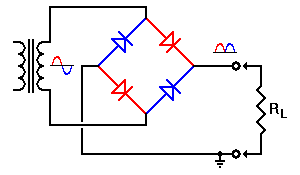
\includegraphics[width=0.99\textwidth]{Images/rectifier.png}}
  \caption{Full-bridge rectifier}
\endminipage\hfill
\minipage{0.32\textwidth}
  \fbox{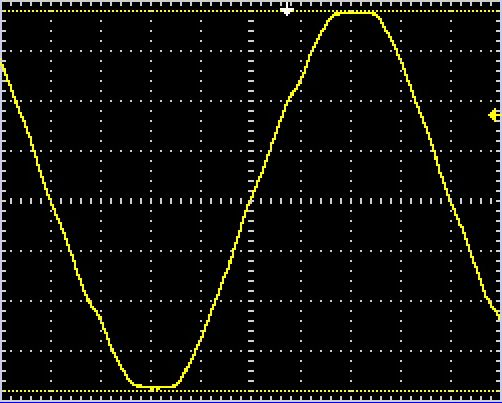
\includegraphics[width=\textwidth]{transformer_output.JPG}}
  \caption{AC input voltage}
\endminipage\hfill
\minipage{0.32\textwidth}%
  \fbox{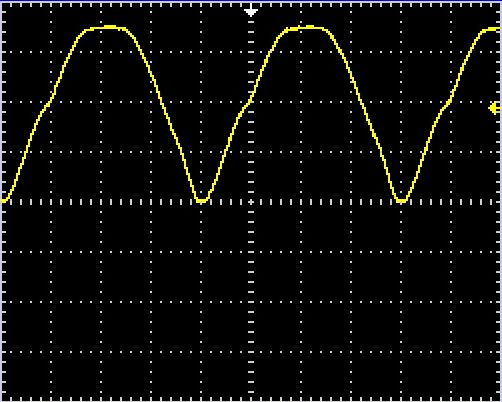
\includegraphics[width=\textwidth]{rectifier_output.JPG}}
  \caption{DC output voltage}
\endminipage
\end{figure}

\subsubsection{DC Filter}

For the output of our power supply we require a constant DC voltage. However after passing through the rectifier circuit the signal still resembles the original sinusoidal signal with large peaks and troths. In order to remedy this, the signal will be filtered.

Filtering is achieved by attaching a single capacitor between the the DC output and ground. This capacitor will charge while the voltage rises, and then discharge as the voltage begins to dip, effectively bridging the peaks of the input sinusoidal signal.

\begin{figure}[!htb]
\minipage{0.32\textwidth}
  \fbox{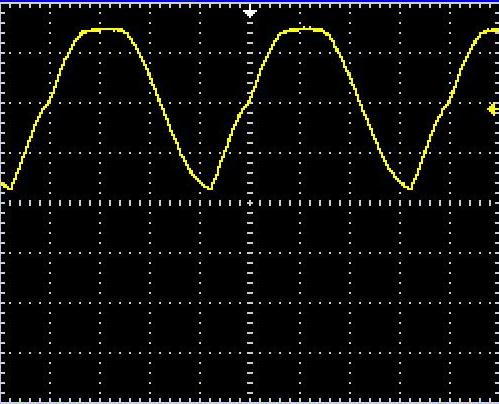
\includegraphics[width=0.98\textwidth]{Rectifier_out_different_cap_values/1uF_cap_rectifier1.JPG}}
  \caption{1uF capacitor}
\endminipage\hfill
\minipage{0.32\textwidth}
  \fbox{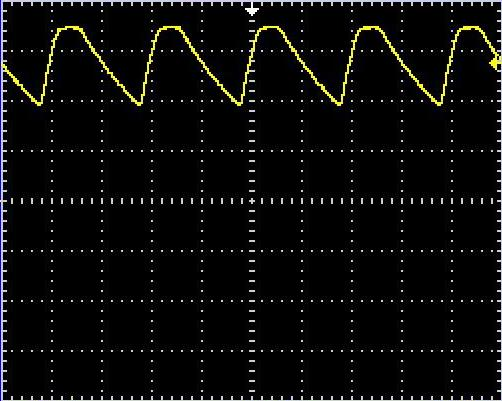
\includegraphics[width=0.98\textwidth]{Rectifier_out_different_cap_values/10uF_cap_rectifier1.JPG}}
  \caption{10uF capacitor}
\endminipage\hfill
\minipage{0.32\textwidth}%
  \fbox{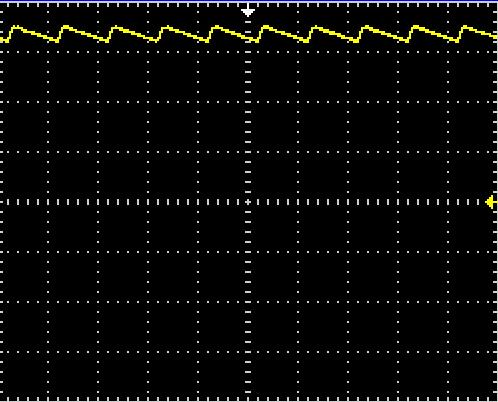
\includegraphics[width=0.98\textwidth]{Rectifier_out_different_cap_values/100uF_cap_rectifier1.JPG}}
  \caption{100uF capacitor}
\endminipage
\end{figure}

Figures 5, 6, and 7 show the output when filtered by different sized capacitors. As the size of the capacitor increases, more charge can be held by the capacitor, thereby filtering out more of the oscillation. It can be noted that it is only important to maintain a voltage above 6V, meaning that even the 10uF capacitor would be viable, however this is also load dependant.

\subsubsection{Voltage regulation and smoothing}

After Smoothing, a clean DC voltage will be output, however it will not be the required voltage and must be regulated to 5V. This can be achieved using zener diodes, linear voltage regulators, or a switch mode power supply. In this project we will use a linear voltage regulator as it will provide a more stable output as the load varies when compared to a zener diode, and its simplicity compared to the switch mode power supply.

However the linear voltage regulator does come with some trade-off's. Most notable are its limited current output, and its inefficiency. The input voltage to the regulator will be truncated, with all excess voltage being dissipated in the form of heat.

Finally the output of the regulator will have a second smoothing capacitor attached between it and ground. This capacitor functions very similarly the the filter cap, removing any irregularities in output voltage, but also serves to help with maintaining constant voltage with varying loads.

\section{Design}
\subsection{Final design specifications and trade-off's}

The final design requirements specify the use of a L7805 5V linear voltage regulator, and 4 1N4007 diodes for rectification. Because of this, the voltage rectification and regulation methods are already predetermined. This allows us to select the filter and smoothing capacitors that will best fit our design requirements.
 
A selection of capacitors ranging from 1nF - 1000nF were tested for filtering the output of the rectifier (this is elaborated upon in the following section). It was concluded that a 10nF capacitor was sufficient for a 1k$\Omega$ load, however serious output ripple could be observed for loads lower than this. Because of this a filter capacitor size of 100nF was used in the final design. A capacitor of the same size was then chosen for output smoothing, This choice was made due to its relative unimportance in our use case of a static load, and for the simplicity of manufacturing. 

The major trade-off of this design is its efficiency. Our AC input was measured to have an RMS voltage of 13.34V, giving a DV voltage of 17.2V after rectification and smoothing. Given the design specifications of a 400mA max current through the transformer, and an output of exactly 5V DC, our regulator will have a calculated worst case efficiency of 29\%, dissipating a total of 4.8W. It is clear that that the use of this regulator limits out overall efficiency, with all excess energy being wasted. A possible replacement for this component would be a switch mode power supply, as these typically feature efficiencies of 70-80\%. This solution however would come with its own trade-off's, these supply are more expensive to build/buy, are more complex in nature, and are also noisy, introducing high frequency electrical noise to a circuit.

Another trade-off of this design are its filter and smoothing caps. the caps that have been chosen are suitable for static loads with small current draw, however if a non static load were to be attached, the filter and smoothing capacitors would discharge faster to compensate for the larger current draw. The solution to this issue would be to use larger filter capacitors, however for our use case, 10nF is sufficient. 

\subsection{Design replication}

\begin{figure}[h]
\hspace{-23pt}
  \fbox{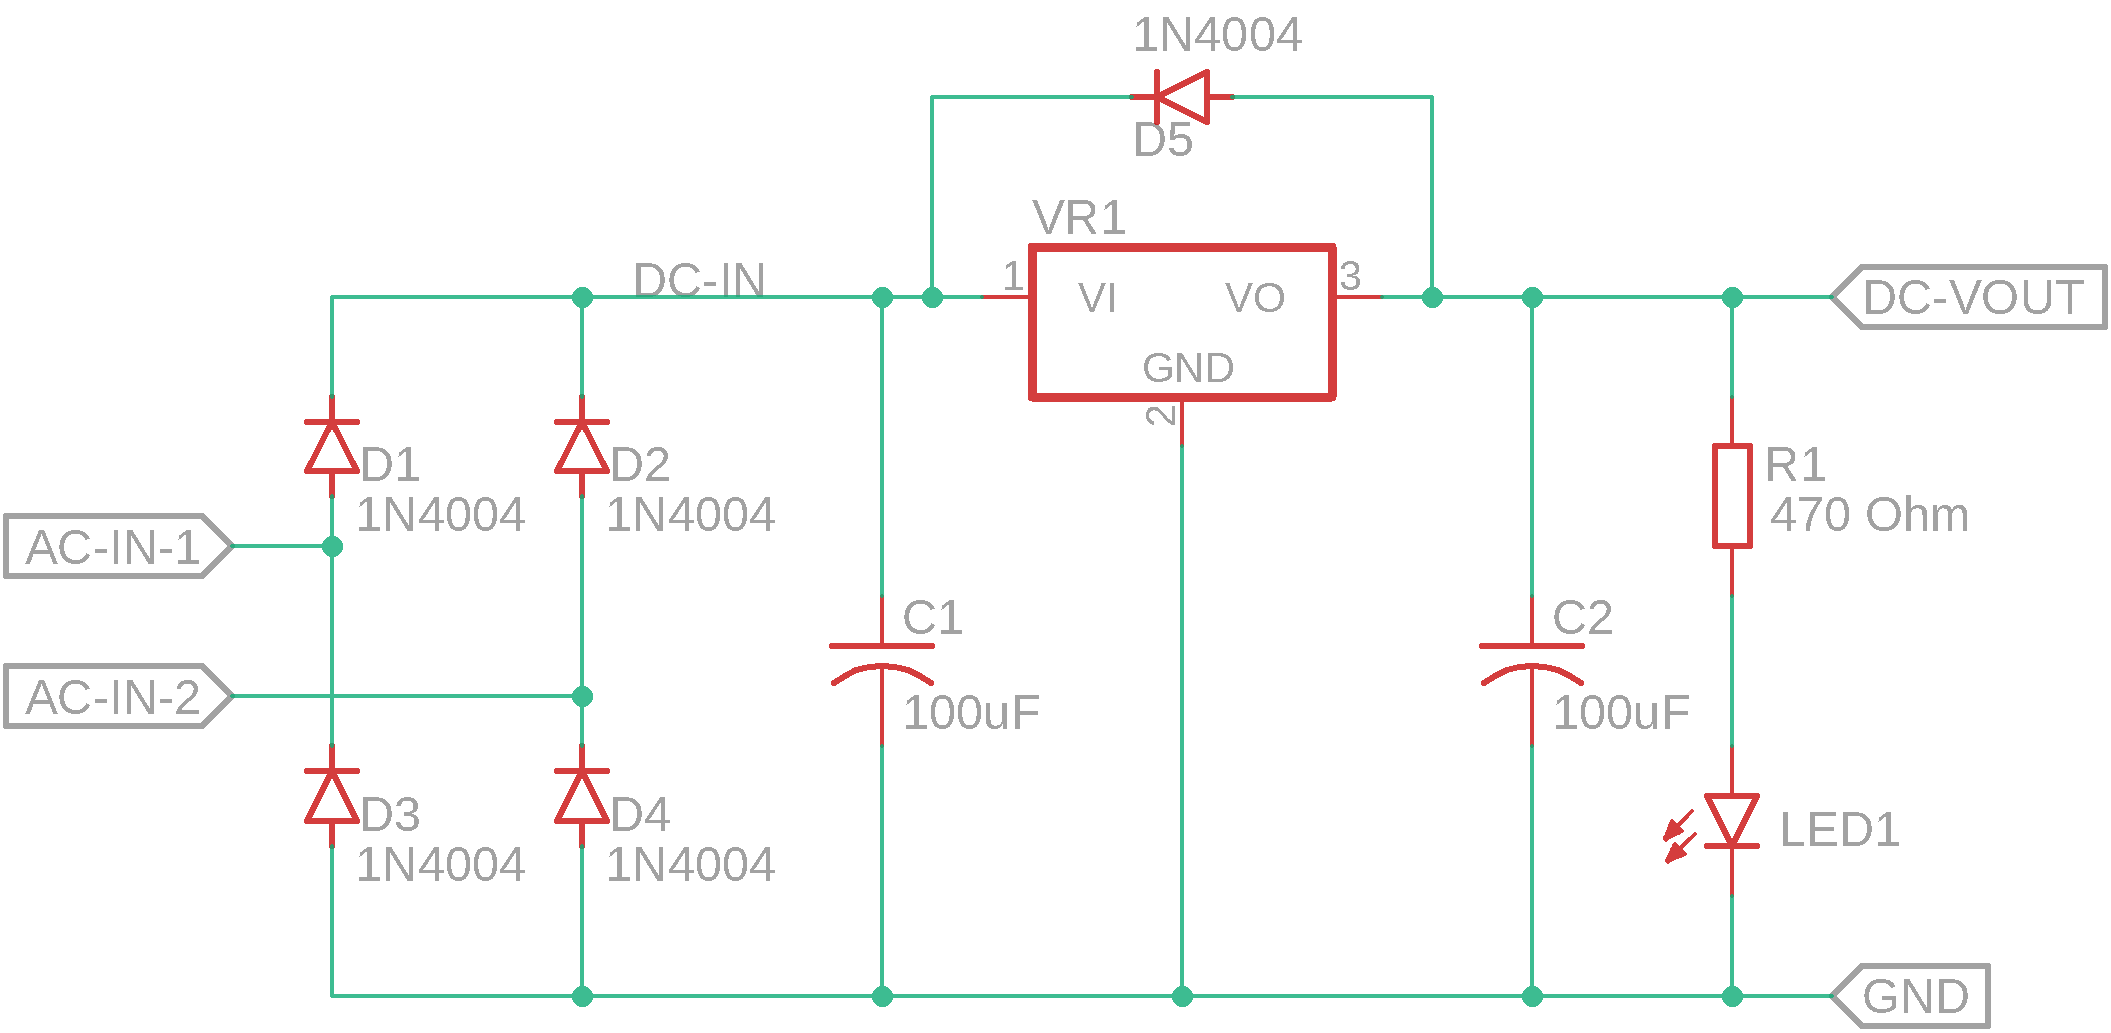
\includegraphics[width = 0.66\textwidth]{Images/Circuit.png}
  		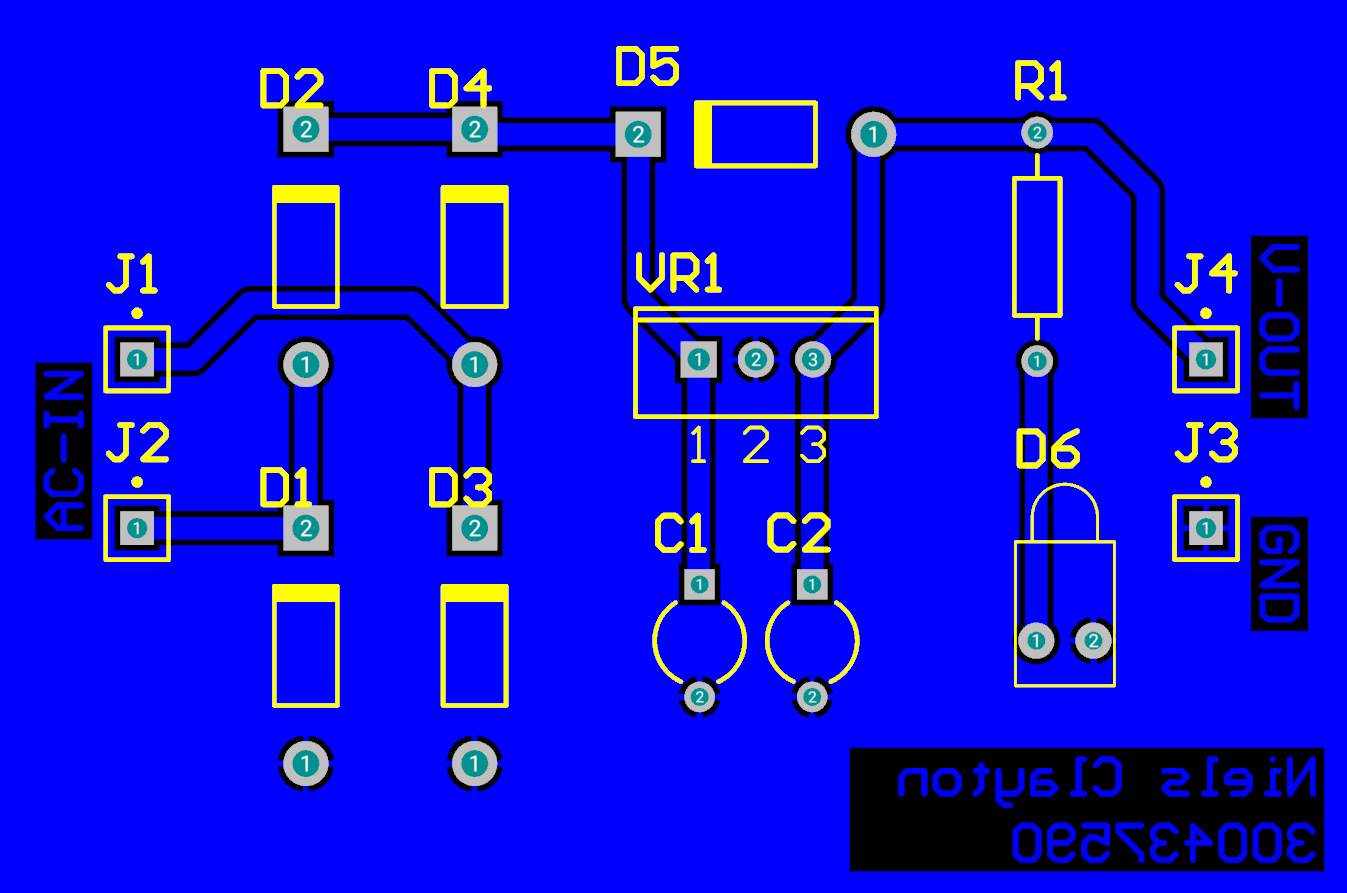
\includegraphics[width = 0.40\textwidth]{Images/PCB.png}}
  \caption{Final circuit design of the power supply and PCB}

\end{figure}
\pagebreak

\section{Circuit construction and testing}

\subsection{Breadboard testing}

Before the construction and milling of the final PCB circuit, the design was re-created on a breadboard testing station to ensure that all the specifications of the circuit were met. We analysed the ripple from the output of the full bridge rectifier with differing filter capacitor values from 1uF - 1000uF. We also observed the loading affect on this rectifier as differing load sizes were tested with a static capacitor value.


\begin{figure}[h]
 \begin{center}
  \fbox{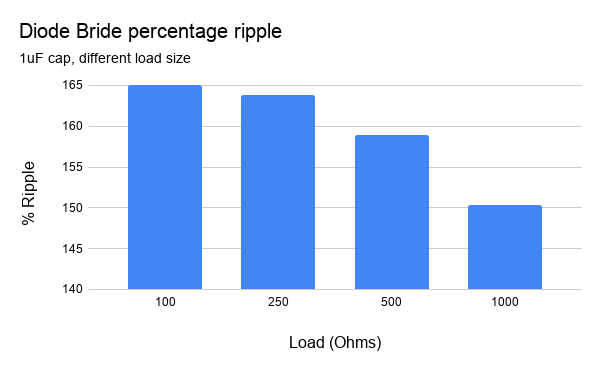
\includegraphics[width=0.5\textwidth]{Images/load_ripple.png}
		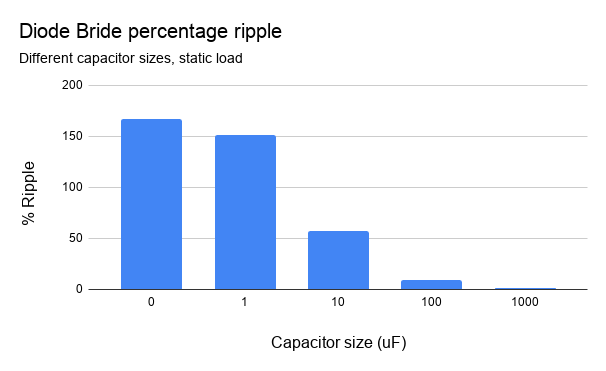
\includegraphics[width=0.5\textwidth]{Images/filter_ripple.png}}
  \caption{Diode bridge percentage ripple}
 \end{center}
\end{figure}

It can be seen from figure 9 that as the size of the filtering capacitors increases, the percentage of ripple form the output of the diode bride decreases drastically. It can also be seen that by increasing the size of the load, the percentage ripple will also decrease. this is do to the filtering capacitor discharging slower when the load is larger as the current draw will be smaller.

It was also important to confirm the output of the regulator at this stage, so we tested the output of the voltage regulator at a series of different input voltages and loads as shown in figure 10. 

\begin{figure}[h]
 \begin{center}
  \fbox{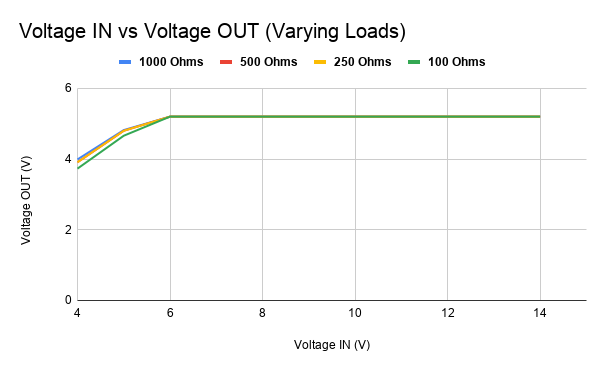
\includegraphics[width = 0.75\textwidth]{Images/v_in_out.png}}
  \caption{Voltage input $\rightarrow$ output curves of the L7805 5V linear voltage regulator}
 \end{center}
\end{figure}

In figure 10 it can be observed that independent of load, as soon as an input voltage of 6V is achieved, there will be a stable 5V output. 


\subsection{PCB design construction and testing}

Once you have etched your PCB, all that is left to do is to build your circuit and complete some final tests. To do this, a soldering iron will be used to attach each of the components to the circuit board in the same configuration as your circuit design. Both sides of the completed circuit board can be seen in figure 11. 

\begin{figure}[h]
 \begin{center}
  \fbox{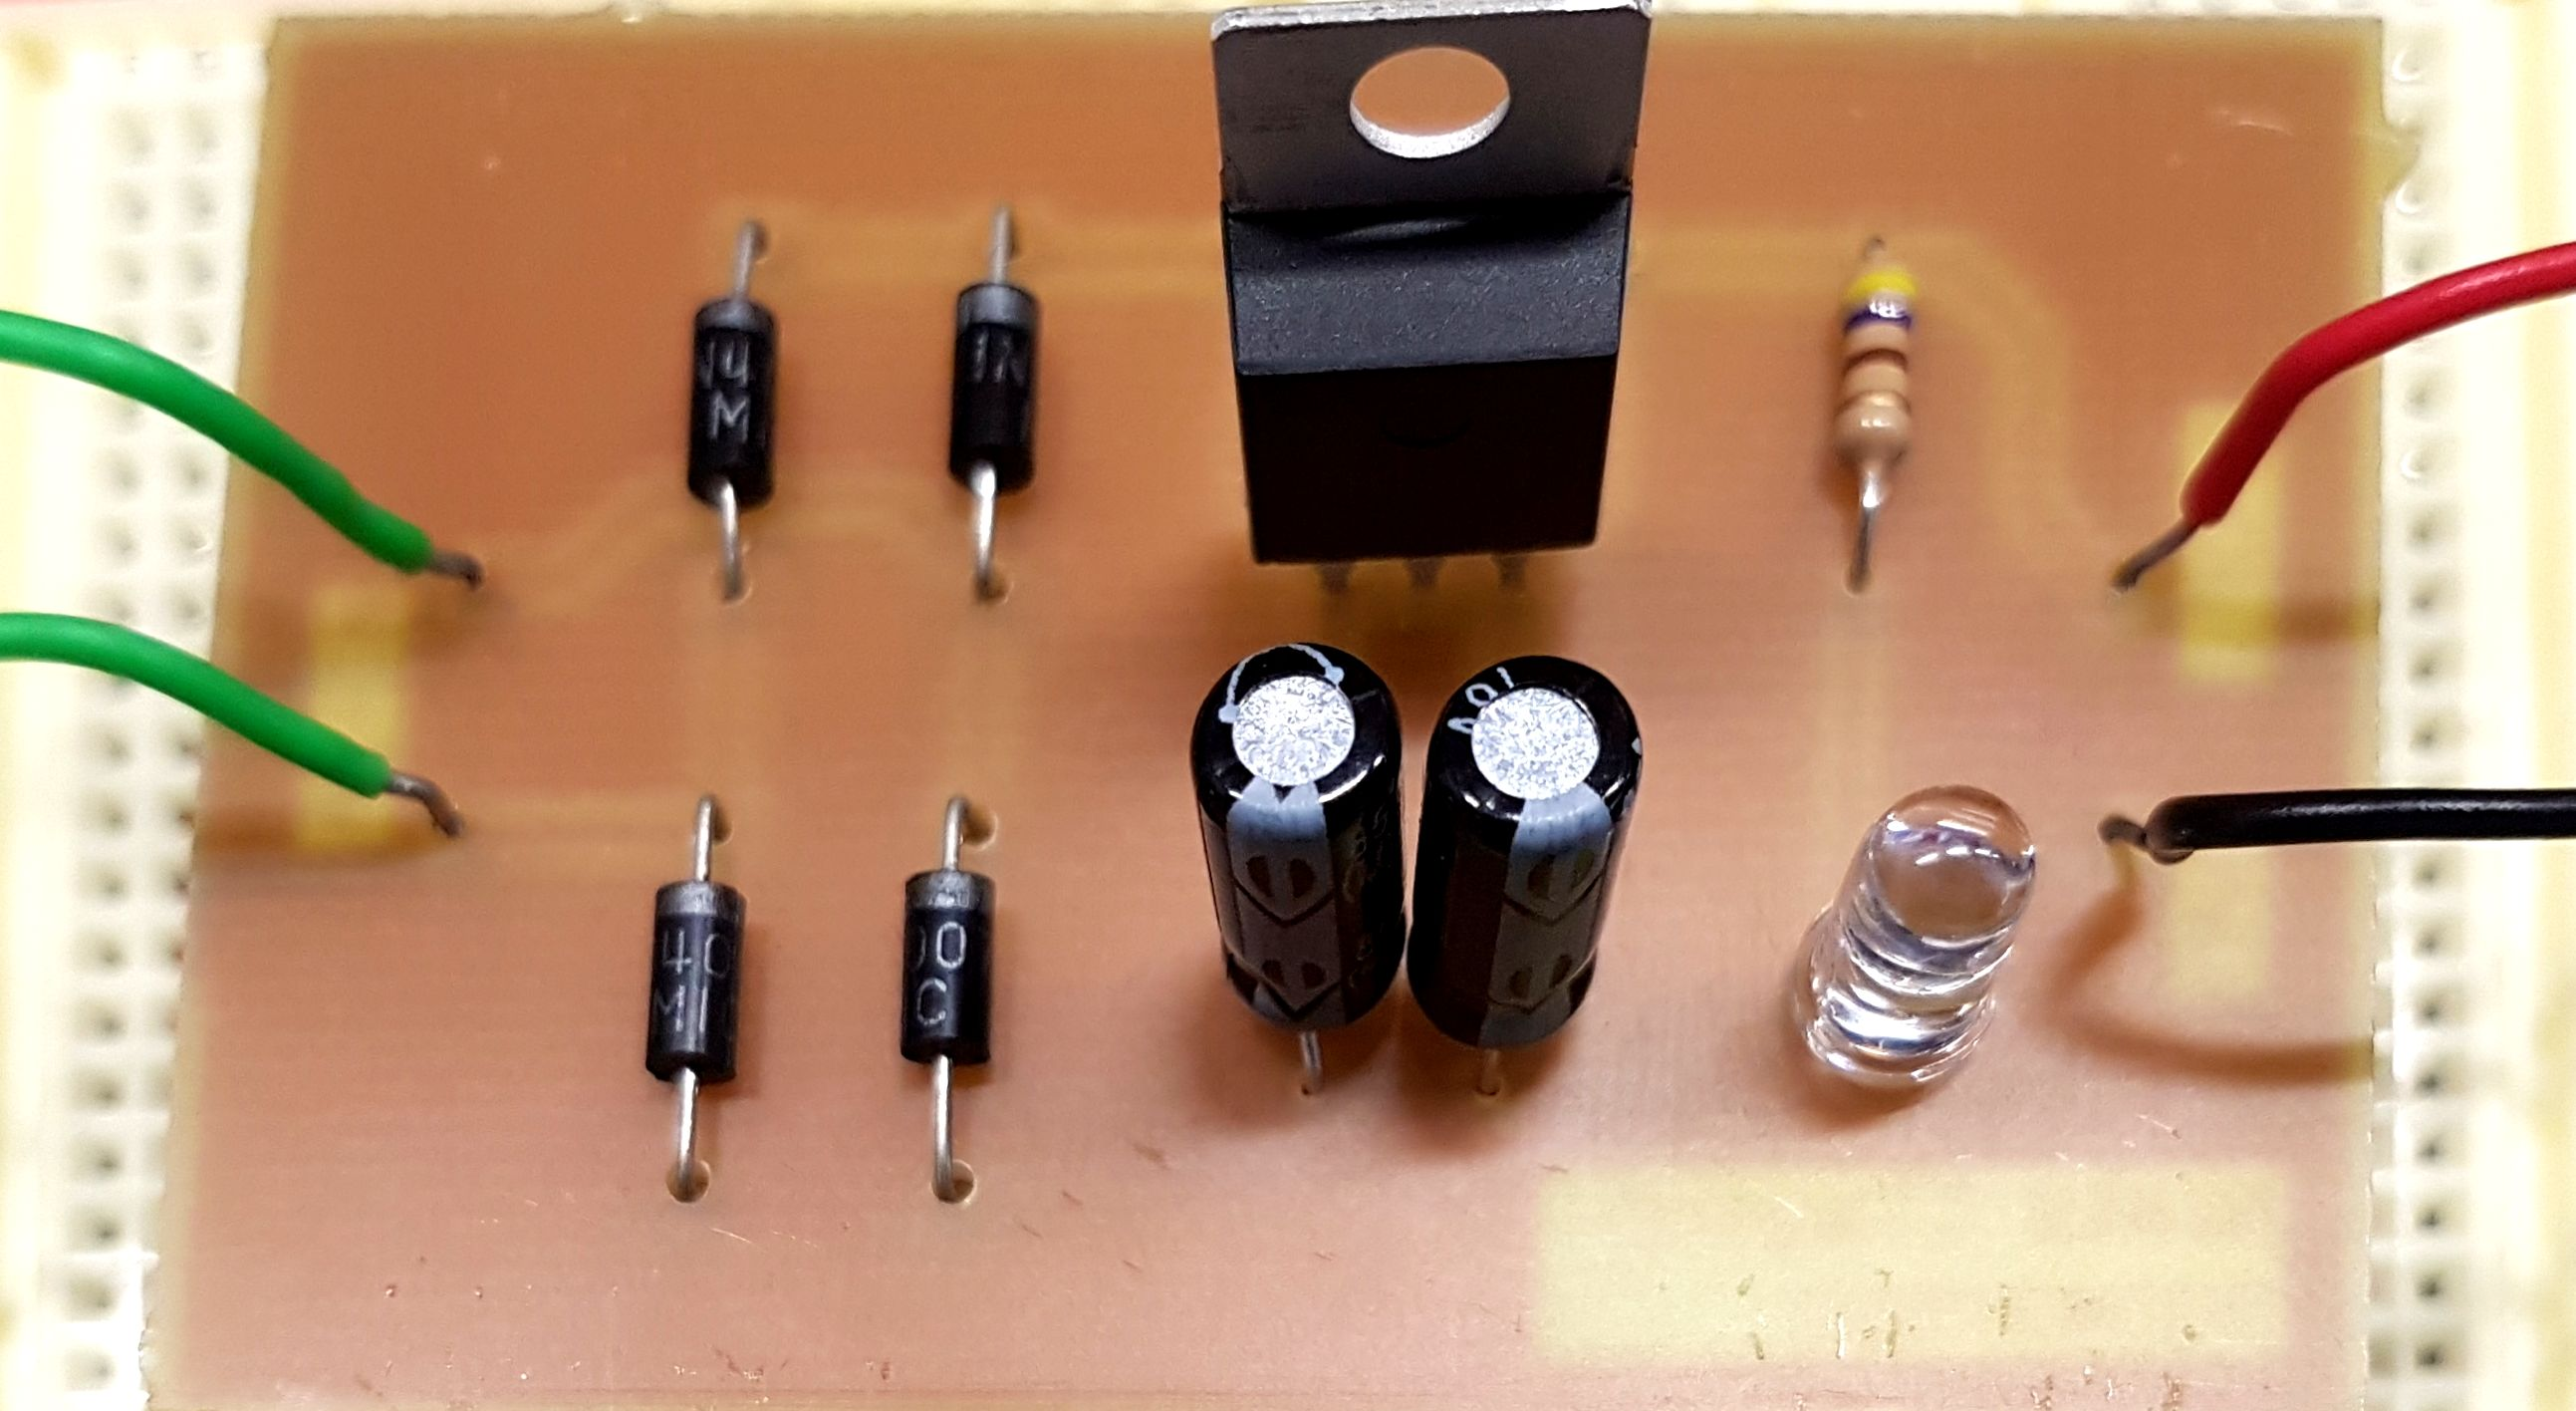
\includegraphics[width=0.5\textwidth]{Images/circuit_top.jpg}
		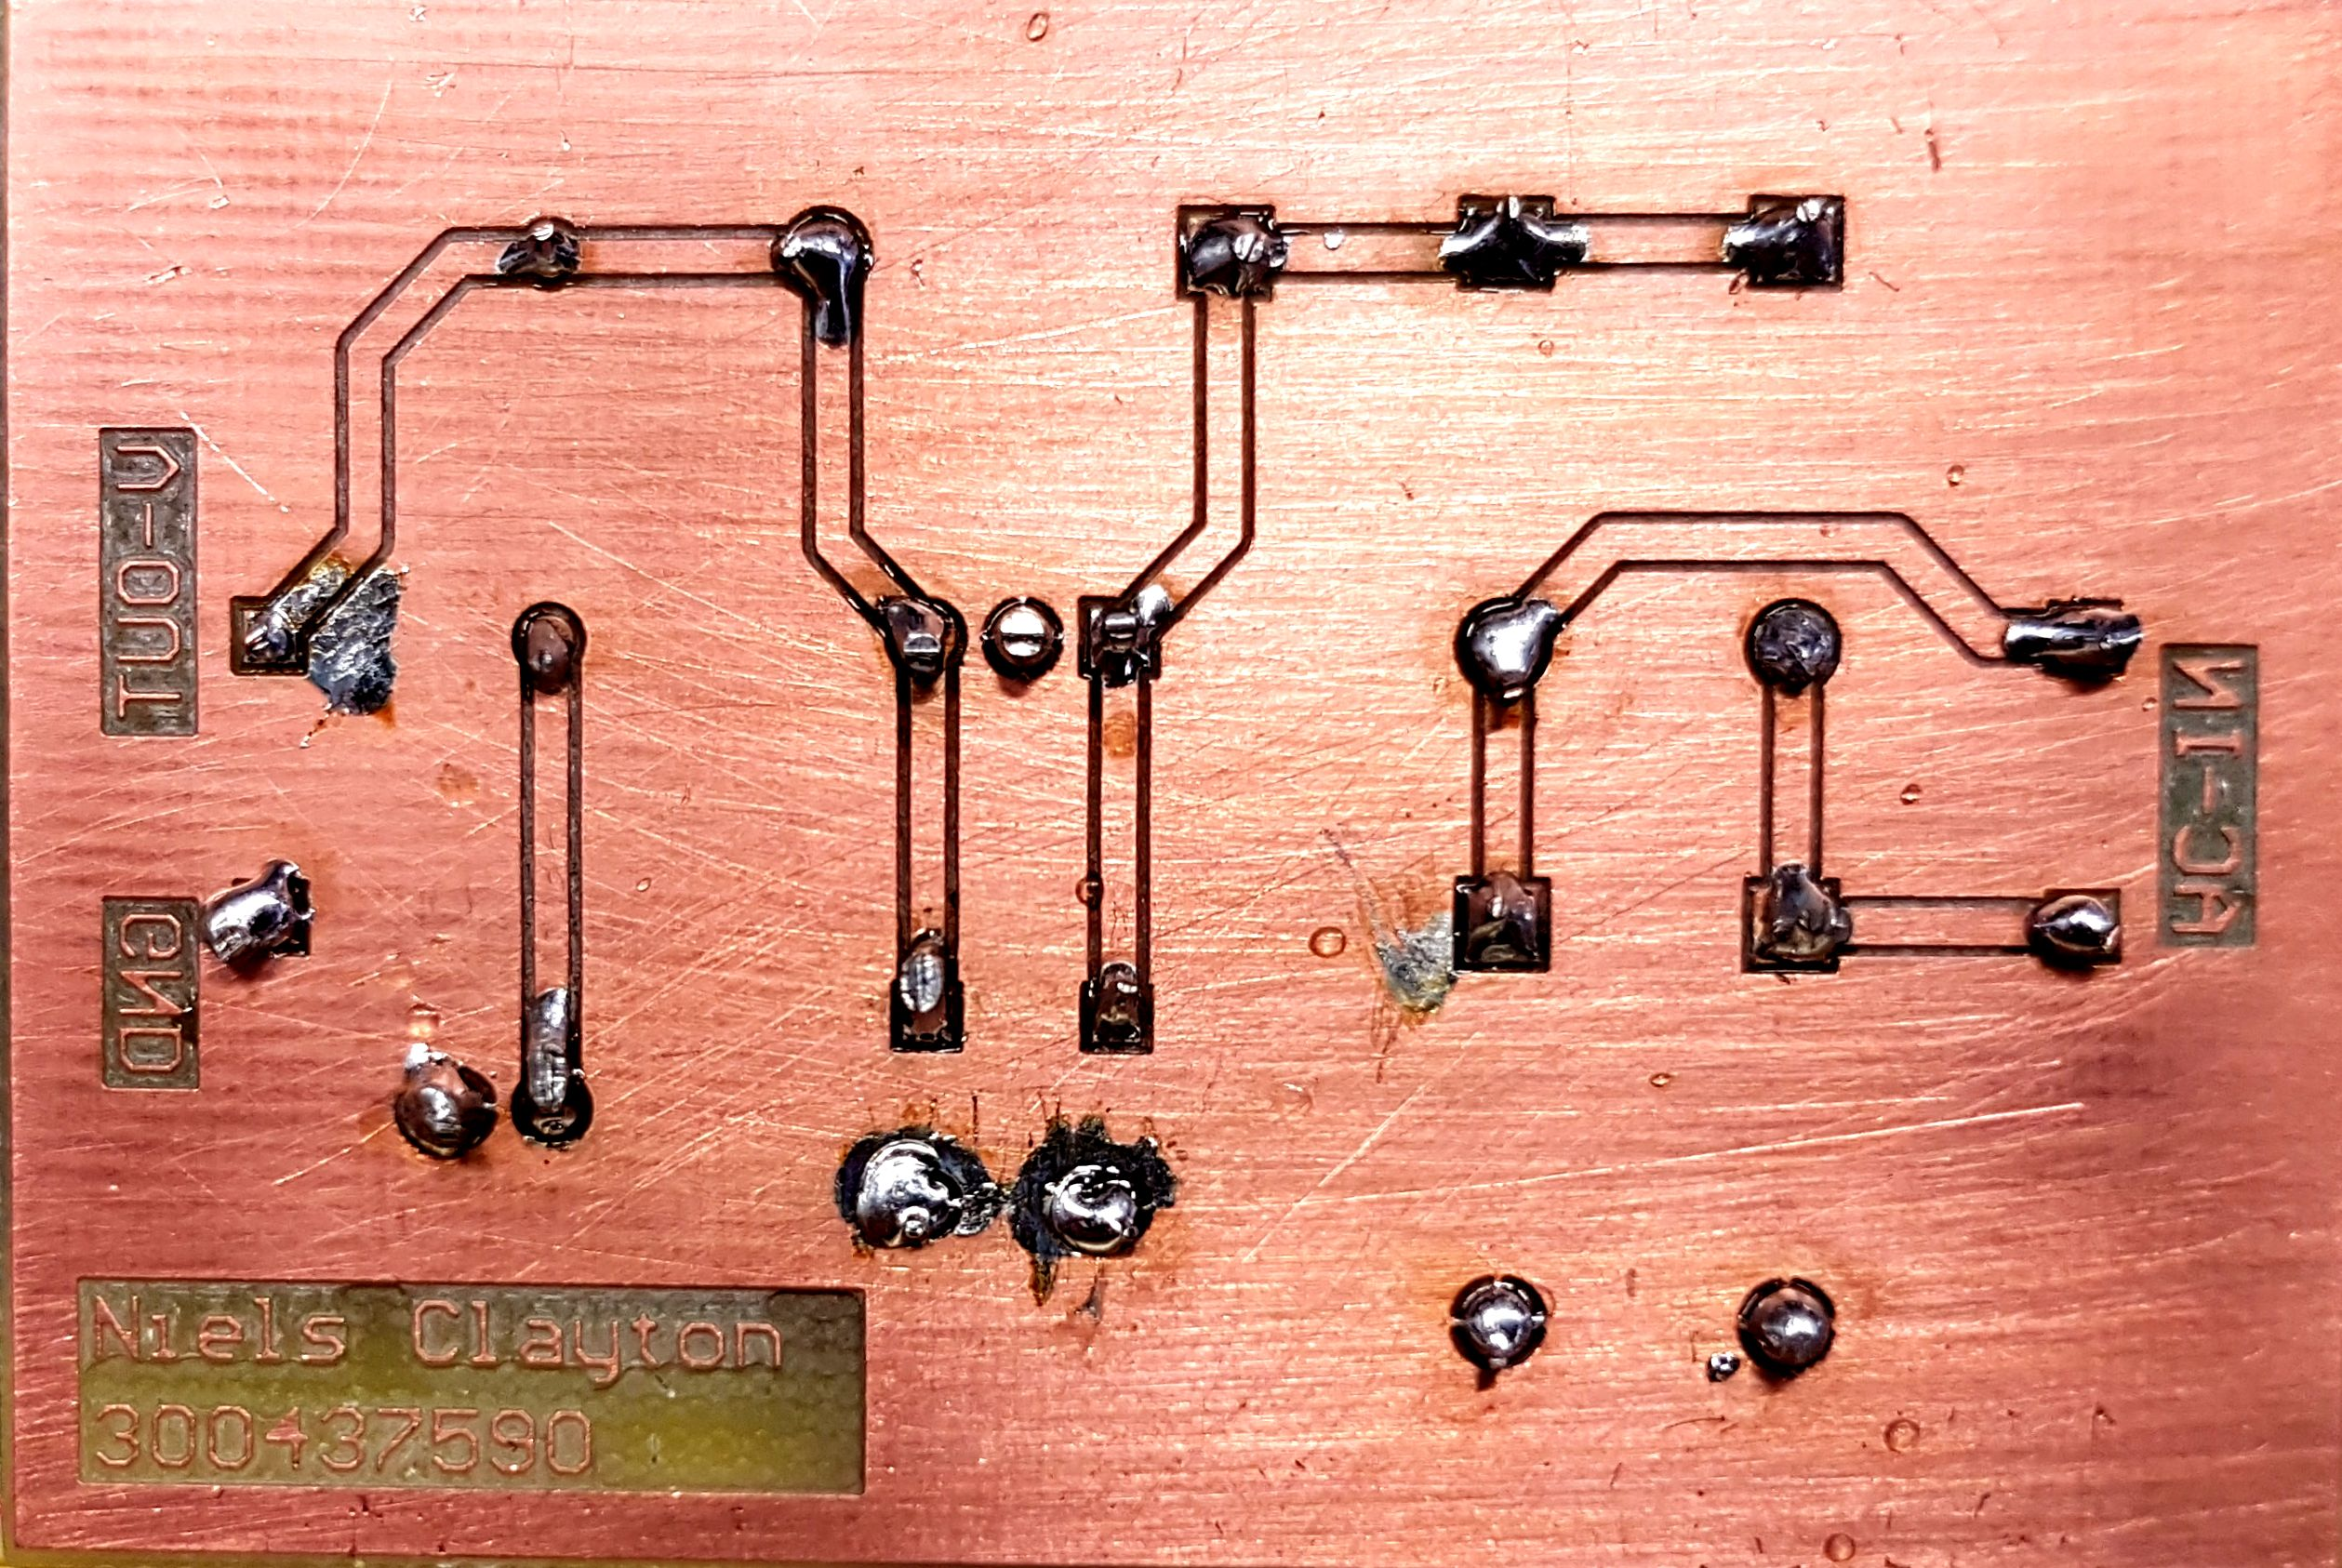
\includegraphics[width=0.5\textwidth]{Images/circuit_bottom.jpg}}
  \caption{Final assembled PCB design of the power supply}
 \end{center}
\end{figure}

For the final testing of the circuit, we will verify that with the 13.34V RMS input, we achieve a steady 5V DC out. We will also look at the ripple of the final circuit with a series of loads, this will ascertain the minimum load the circuit will be able to reliably supply, as well as the maximum current output of our final PCB. 

\begin{center}
\begin{tabular}{|c|c|c|c|c|}  
\hline
\(\displaystyle I_{IN} (mA) \) & \(\displaystyle I_{OUT} (mA) \)  & \(\displaystyle V_{OUT} \) & Load \(\displaystyle \Omega \) & \(\displaystyle V_{P-P} \)\\
\hline
66.7  & 42   & 4.4  & 100 & 3.4\\
47.9  & 23   & 4.8  & 200 & 2.12\\
39.6  & 16   & 4.96 & 300 & 1.08  \\
34.6  & 12.2 & 5    & 400 & 0.22\\
29.4  & 8.3  & 5    & 500 & 0.08 \\
\hline
\end{tabular}
\end{center}


\begin{figure}[h]
 \begin{center}
  \fbox{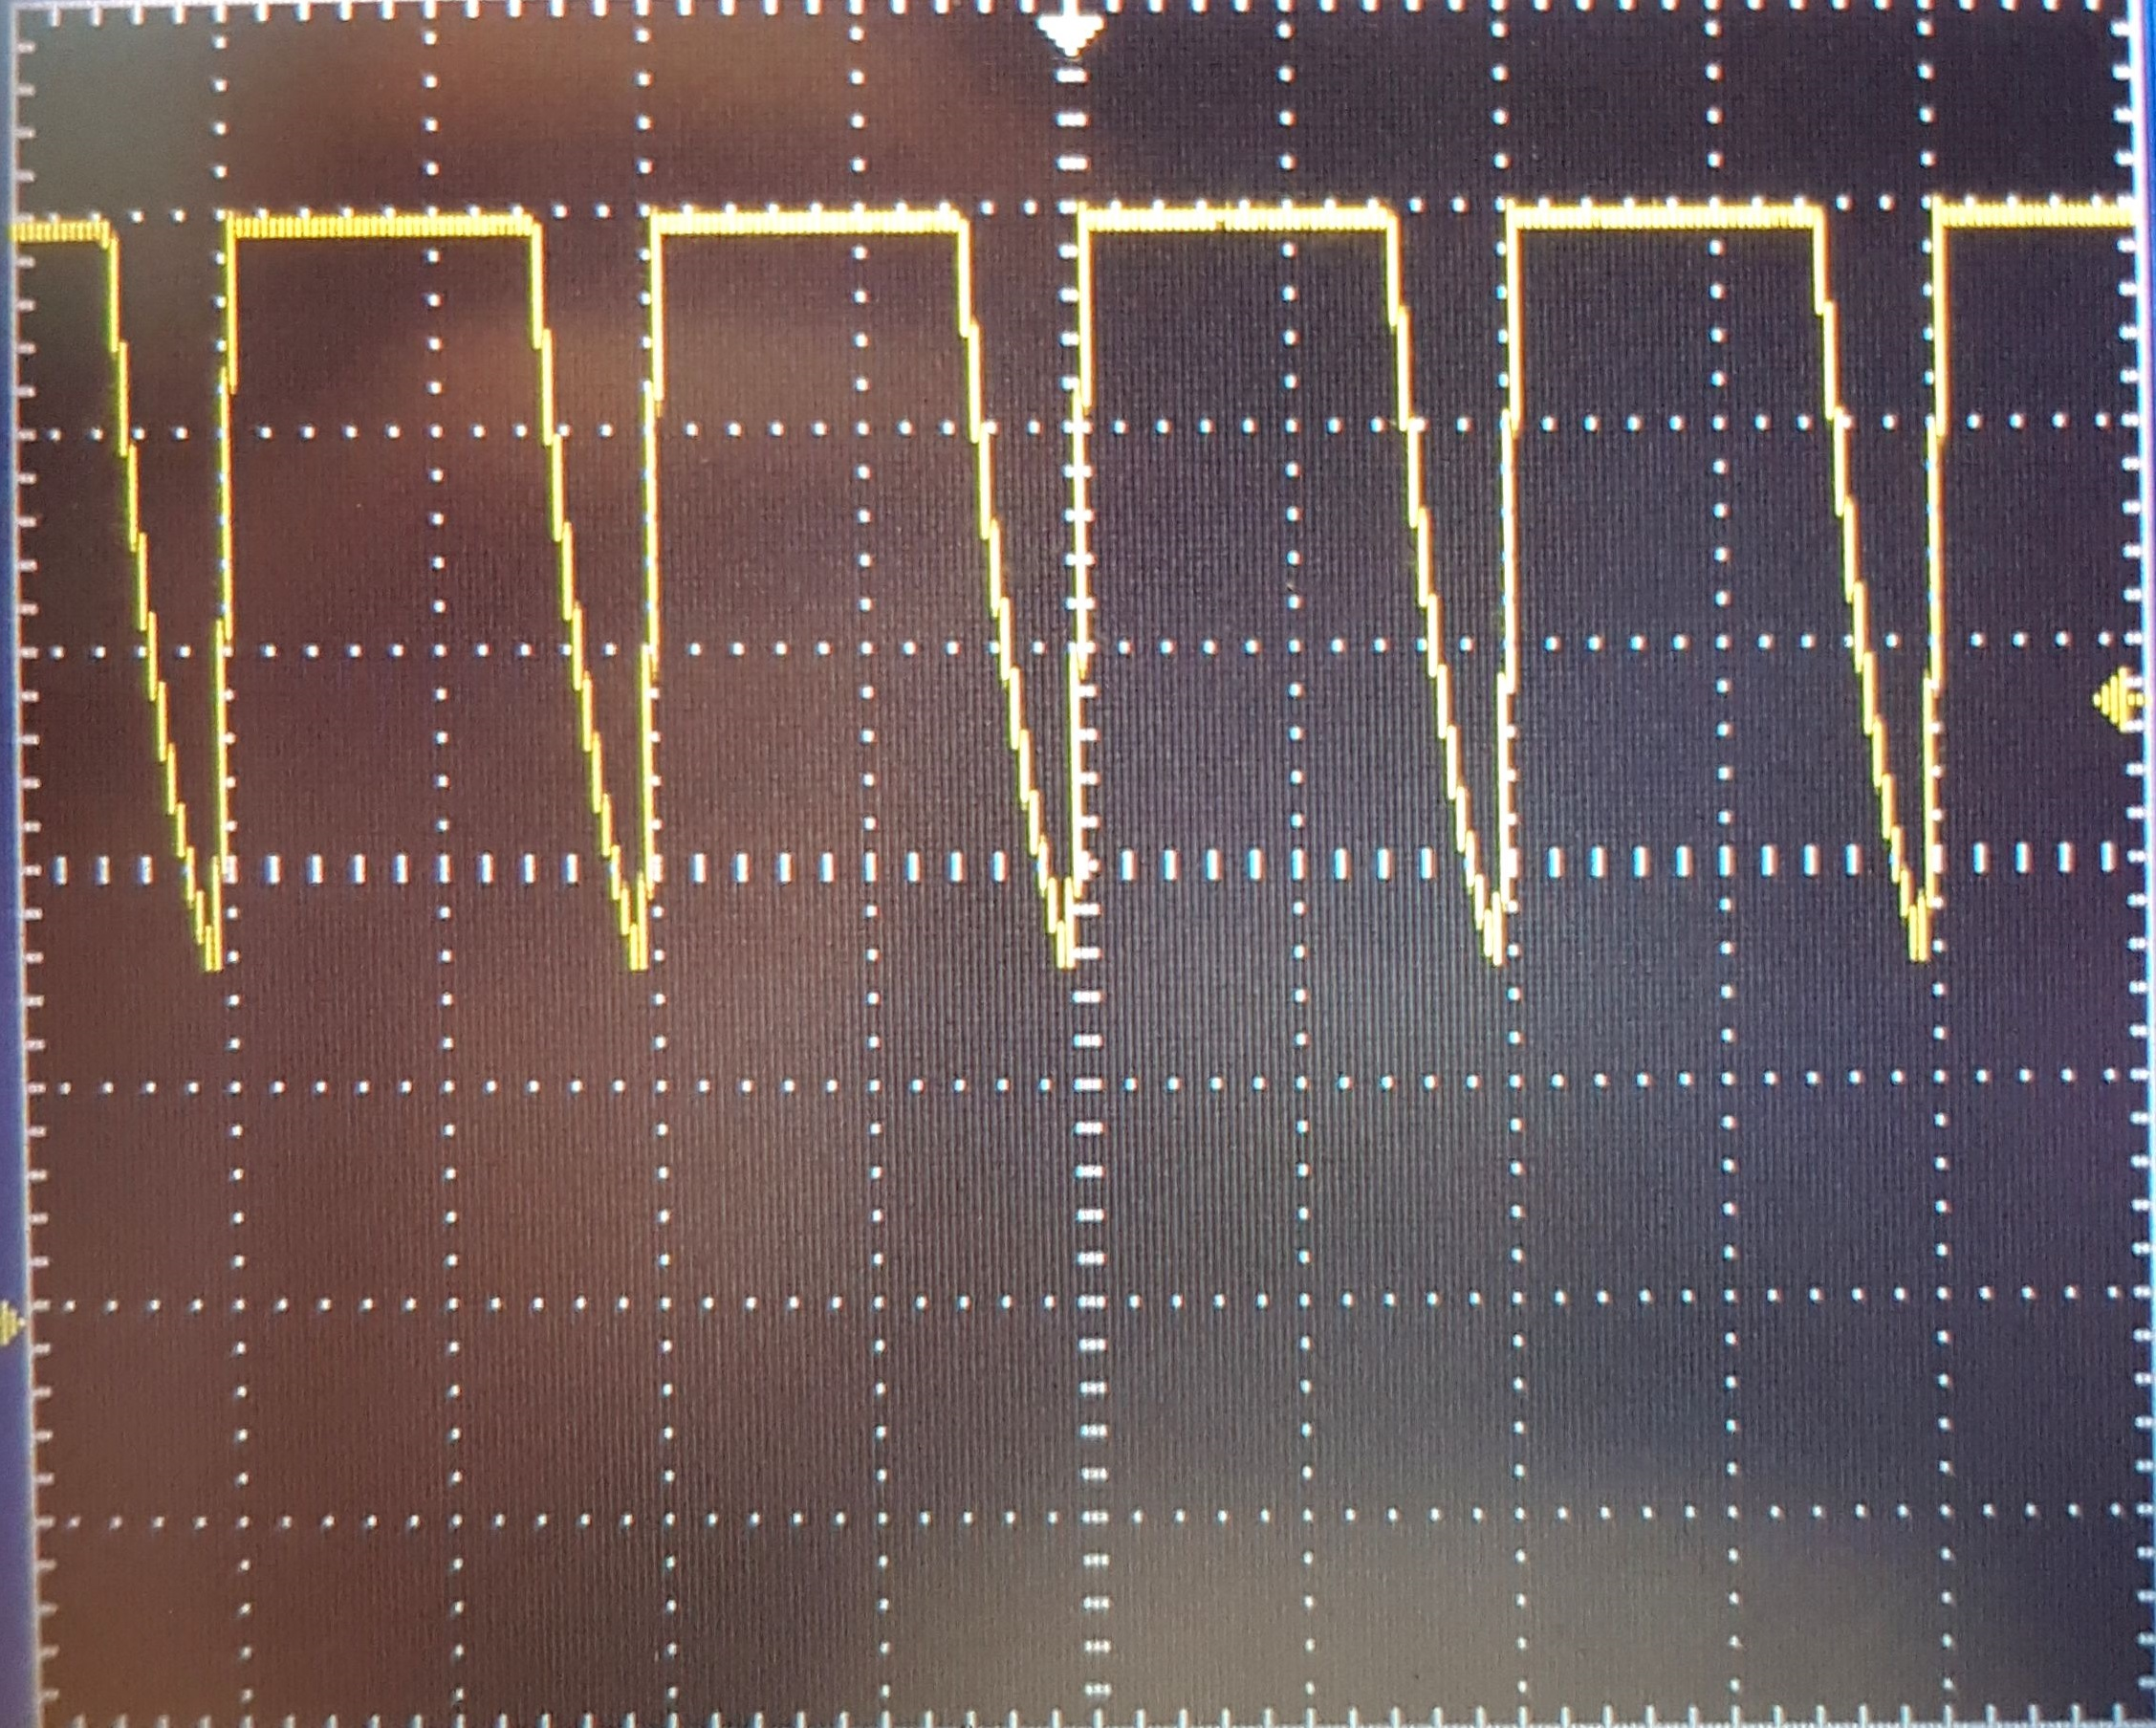
\includegraphics[width=0.25\textwidth]{Images/100.jpg}
		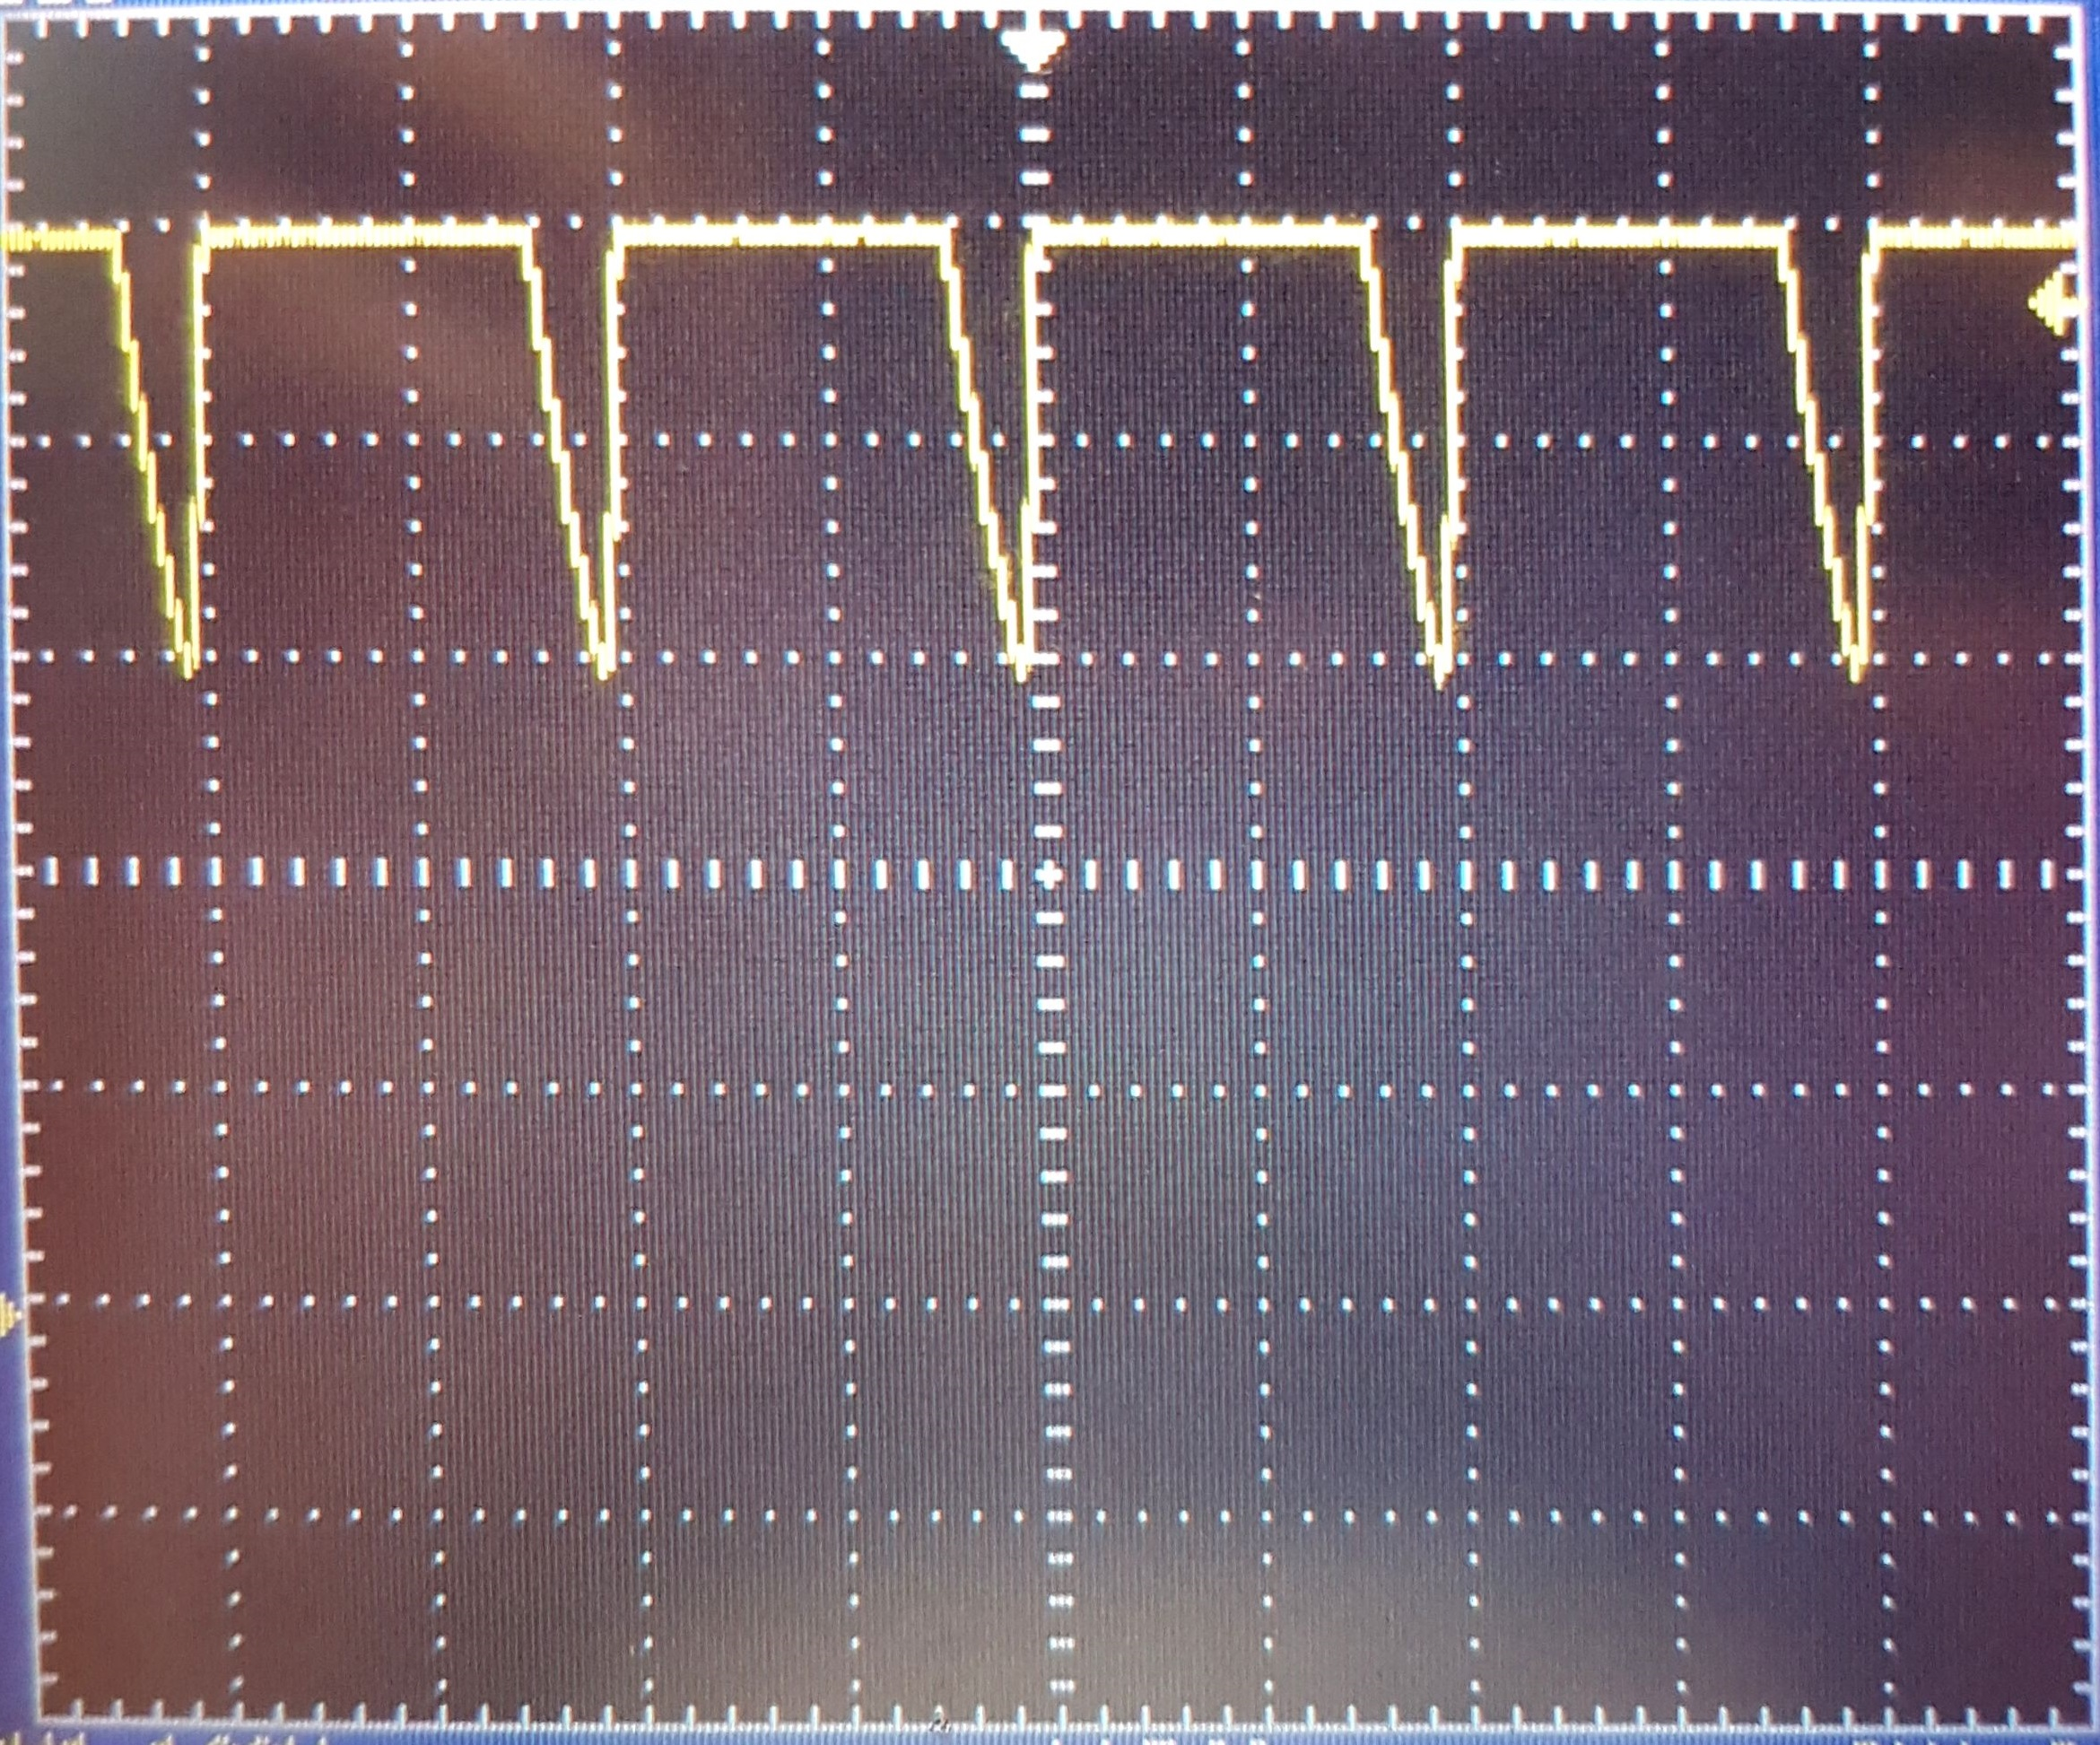
\includegraphics[width=0.25\textwidth]{Images/200.jpg}
		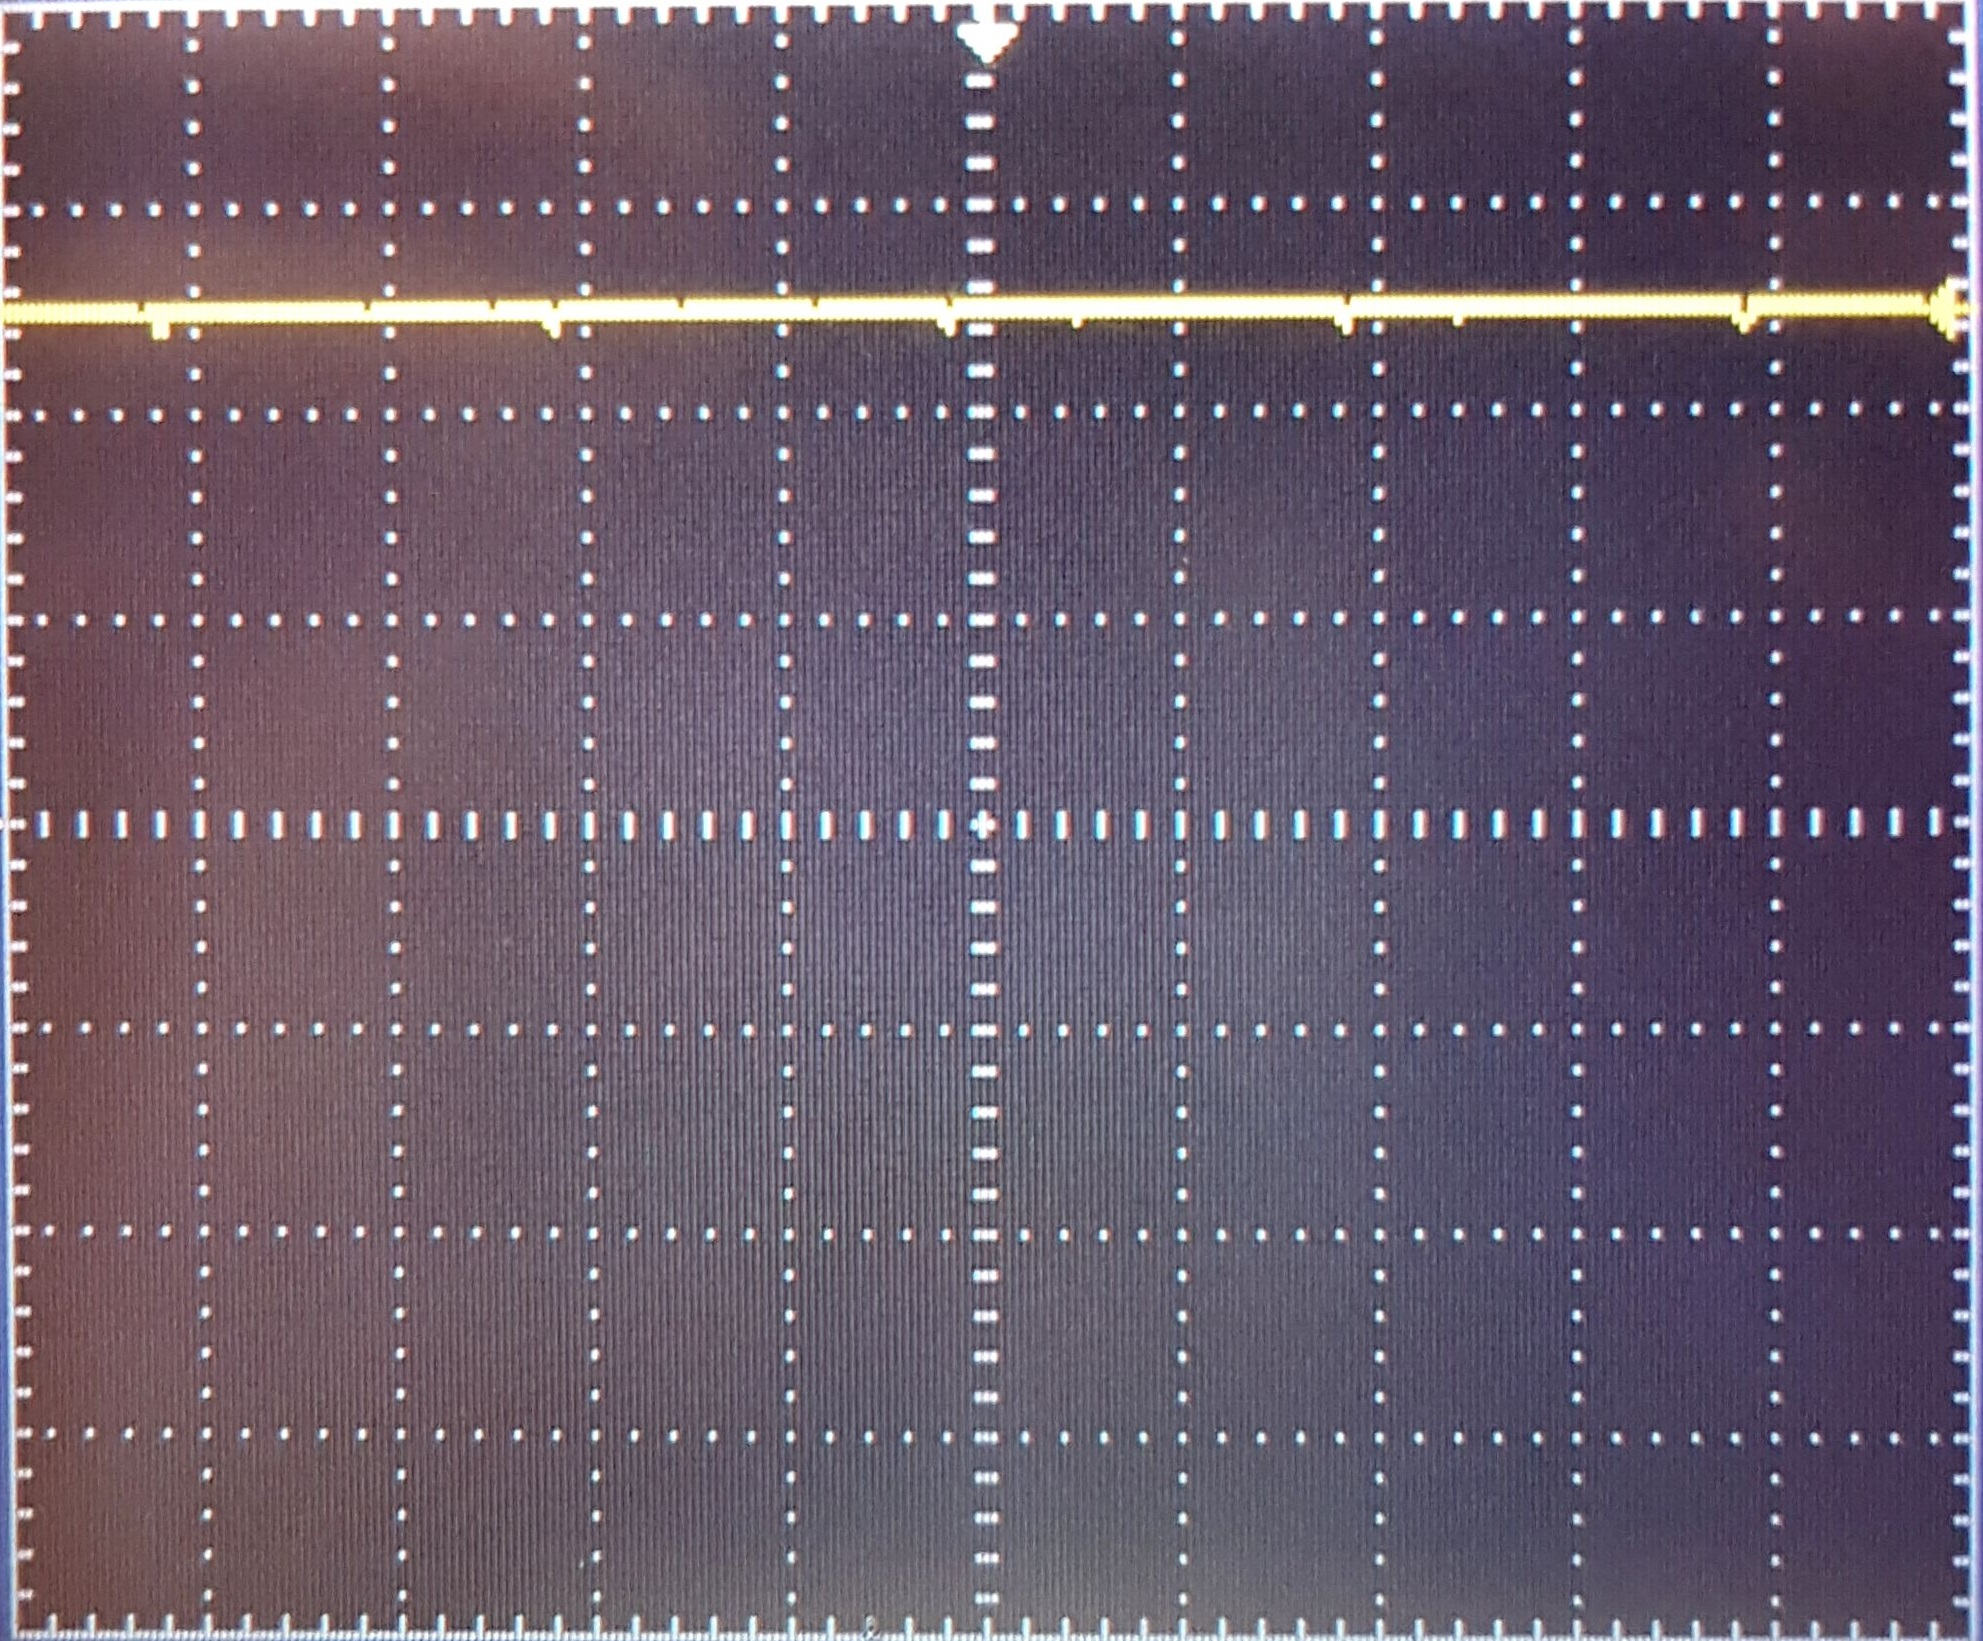
\includegraphics[width=0.25\textwidth]{Images/400.jpg}
		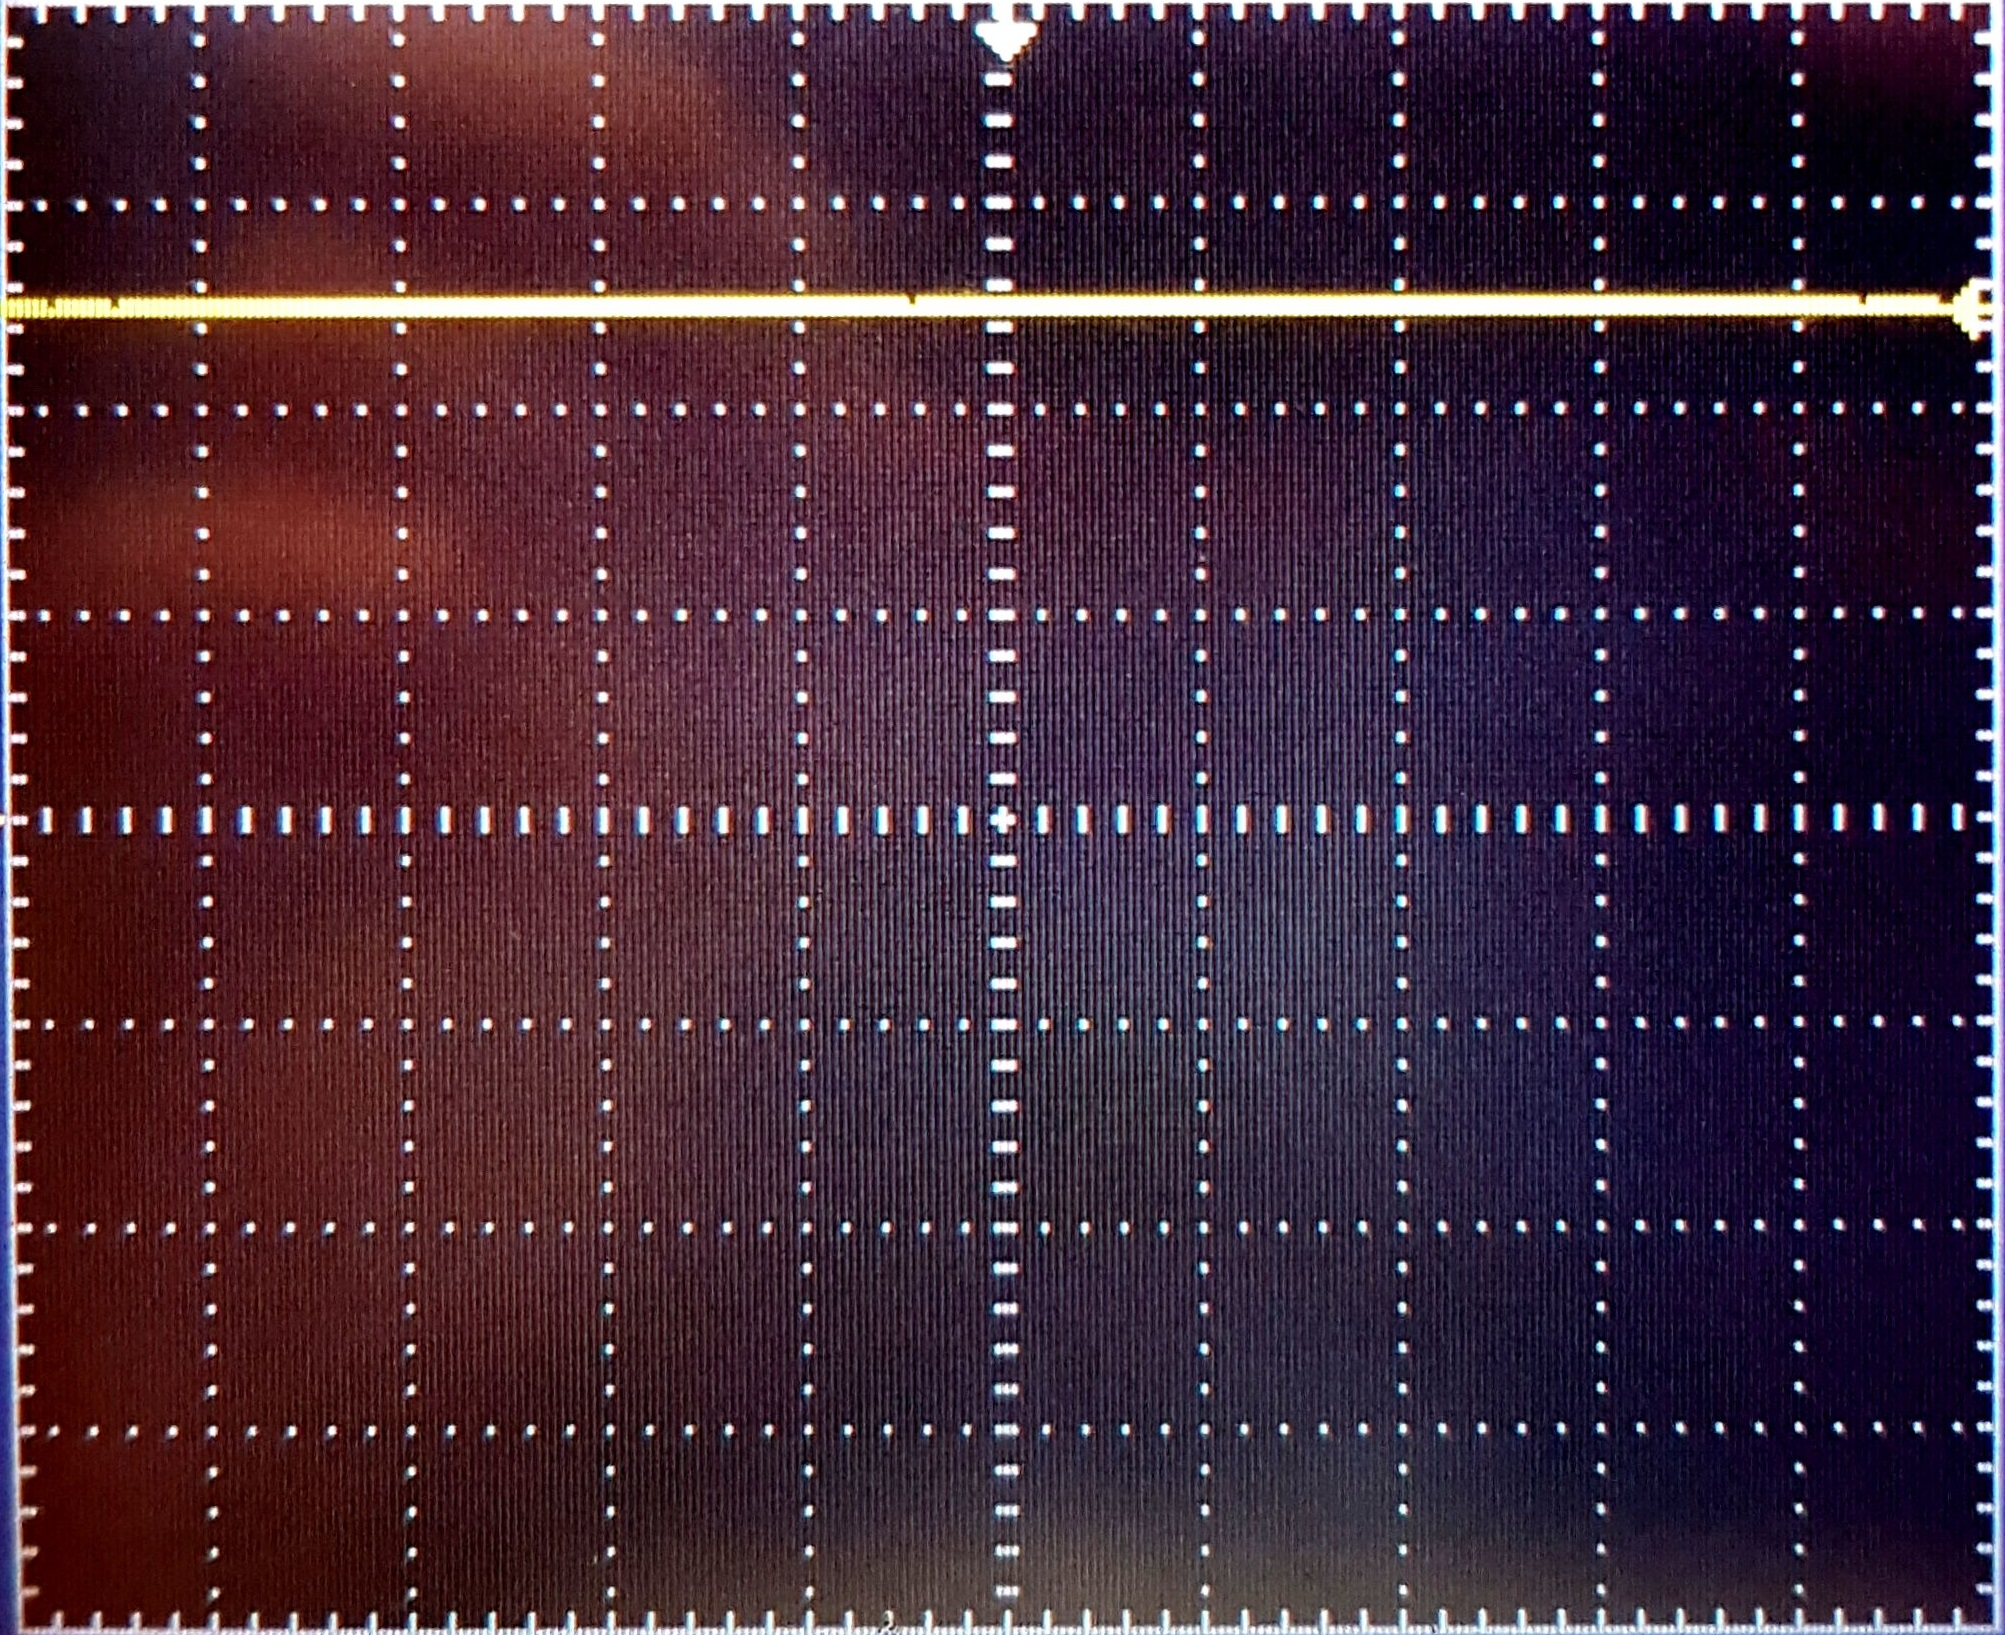
\includegraphics[width=0.25\textwidth]{Images/500.jpg}}
  \caption{Output ripple for loads of 100$\Omega$, 200$\Omega$, 400$\Omega$, 500$\Omega$}
 \end{center}
\end{figure}

From the table above and figure 12, it can be seen that for loads below 400$\Omega$ there is substantial ripple on the output voltage. It can also be seen that for loads below 400$\Omega$ there isn't a stable output voltage of 5V. From this we can see that the minimum load capability of this power supply is 400$\Omega$, giving a maximum current draw of 12.2mA out and 34.6mA on the input of the power supply. 

\pagebreak

\section{Discussion}

Over the course of this project everything went very smoothly, and there were no large issues. In the design stage all components were chosen for us except the size of the filter and smoothing capacitors, making the overall project rather fool proof. For future projects I believe it would be more enjoyable to be given a larger degree of freedom when it comes to the components to use. 

When it comes to the overall design of the power supply, it is very simplistic, and although it does function to rectify and step down an AC input to 5V DC, there are many large drawbacks to this design. The major draw back of our design would be its inefficiency, especially when compared to similar products like a switch-mode power supply (buck converter) that will achieve much higher efficiencies. Another draw back of this design would be the small size of the filter and smoothing capacitors. These capacitors are there to supply voltage when there is a dip in the output of the circuit. the larger the capacitors, the the smaller the load can be before there are signs of output ripple. Larger capacitors will also allow the supply to handle non-static loads.
Overall this project was very enjoyable, and I have learnt a great deal about the operations of basic power supply circuits, I also enjoyed the hands on aspects of this projects like when we got the opportunity to solder for our selves. 

\section{Additional questions}
\subsection*{a)}
If we were to put a solely DC input into our power supply circuit, it would function exactly the same, as long a the input voltage is greater than 7.4V. This is due to the fact that we will no-longer be utilising the full bridge rectifier to rectify the current, but our DC current will still pass through 2 diodes leading to a voltage drop of 1.4V. then the active voltage of the L7805 5V linear voltage regulator is 6V, meaning that we will need 7.4V DC into the supply to have the required 6V after diode drops.

\subsection*{b)}
These capacitors are there to supply voltage when there is a dip in the output of the circuit. For the filter capacitor, it is there to filter out the oscillation  in the rectified DC voltage from the rectifier. The filter cap will charge during the peaks, and then as the voltage dips, the capacitor will discharge, to supply voltage. The smoothing capacitor works in a very similar manor, and will discharge when there are dips in the output voltage.

\subsection*{c)}

\subsubsection*{i)}

Our diode bridge will not be appropriate for this use, this is because each half wave of the signal must pass through 2 diodes, each with a voltage drop of 0.7V. Because of this the input signal wont be able to pass through the bridge as it is not atleast 1.4V peak on each half wave.

\subsubsection*{ii)}

\end{document}



